\section{Aprendizado Semissupervisionado}
    \label{sec:semi-supervised-learning}
    
    %Aprendizado Supervisionado, como mencionado na seção \ref{sec:machine-learning} deste trabalho, é a forma de aprendizado que todos os dados tem uma classe, isso é, para cada instância na base de dados há uma classe relacionada a ela.
    
    Conforme mencionado anteriormente e apresentado na Figura~\ref{fig:machine-learning}, o \ac{ssl} está na interseção dos aprendizados supervisionado e não supervisionado, onde uma parte dos exemplos possui o rótulo e outra não.

    \begin{figure}[h]
        \centering
        \caption{Divisão do Aprendizado.}
        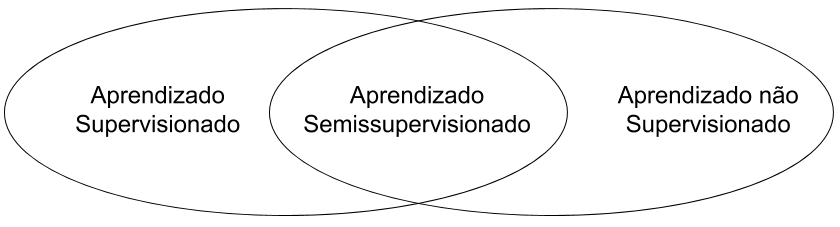
\includegraphics[scale = 0.4]{figuras/Aprendizado-de-maquina.png}
        \source{O Próprio Autor (\imprimirdata)}
        \label{fig:machine-learning}
    \end{figure}
    
    A abordagem Supervisionada exige uma base de dados com todos os exemplos rotulados para gerar um classificador com uma eficácia maior. Porém, a abordagem semissupervisionada vem demonstrando ser relevante para muitas aplicações no mundo real, pois nem sempre é possível obter a base com todos os dados rotulados, ou é necessário utilizar recursos financeiros e conhecimento dos profissionais com a finalidade de treinar um classificador com uma eficácia maior. Então, com o \ac{ssl} reduz\hyp{se} o custo e esforço necessário para executar a rotulagem em um conjunto de dados \cite{bouchachia2012semi, hady2013semi}.
    
    Além disto, essa abordagem pode ser utilizada tanto para as tarefas de classificação como as tarefas de \textit{clustering}. Para a tarefa de classificação, os classificadores são utilizados para realizar predições sobre os dados adicionando no conjunto dos dados rotulados $L$. Quando a tarefa é de \textit{clustering} os exemplos rotulados auxiliarão a definir os núcleos destes agrupamentos, obtendo assim uma eficácia melhor no agrupamento~\cite{chapelle2006semi}.
    
    Dentre os diversos algoritmos do aprendizado semissupervisionado destacam\hyp{se} \textit{Co\hyp{Training}} e \textit{Self\hyp{Training}}~\cite{zhu2008survey}. O \textit{Co\hyp{Training}} tem a sua execução dividindo verticalmente a base de dados $D$ em $D_1$ e $D_2$, de modo que os atributos em $D_1$ são diferentes dos de $D_2$~\cite{blum1998cotraining}.
    
    % com os aprendizes baseados em árvore de decisão, regras de associação, no método bayesiano e instâncias
    
    Neste trabalho será dado um foco maior ao algoritmo \textit{Self\hyp{Training}}, também conhecido por \textit{Self\hyp{Learning}}, \textit{Self\hyp{Labeling}} ou \textit{Decision\hyp{Directed}}. Um algoritmo do \ac{ssl} onde sua execução é dada por: i) iniciar com um conjunto pequeno de dados rotulados; ii) treina o classificador com os exemplos do conjunto dos rotulados $L$; iii) conforme suas previsões realiza a classificação dos exemplos que não possuem classe; iv) adiciona os exemplos no conjunto dos rotulados $L$~\cite{chapelle2006semi, grandvalet2005semi, zhu2009introduction}. No Pseudocódigo~\ref{alg:self-training} encontra-se o algoritmo do \textit{Self\hyp{Training}}.
	
	%% pseudo-código by araujobd
    %
    \begin{algorithm}[H]
        \caption{Pseudocódigo do \textit{Self\hyp{Training}}}
        \label{alg:self-training}
        \SetAlgoLined
        \begin{algorithmic}[1]
            \REQUIRE \textit{dados rotulados} $\{(\mathbf{x}_i, y_i)\}^l_{i = 1}$, \textit{dados não rotulados} $\{\mathbf{x}_j\}^{l+u}_{j=l+1}$
            \ENSURE $L \leftarrow \{(\mathbf{x}_i, y_i)\}^l_{i = 1}$ \textit{e} $U \leftarrow \{\mathbf{x}_j\}^{l+u}_{j = l+1}$
            \REPEAT
            	\STATE \textit{Treinar $f$ de $L$ usando aprendizado supervisionado}
            	\STATE \textit{Aplique $f$ as instâncias não rotuladas em $U$}
            	\STATE \textit{Remova um subconjunto $S$ de $U$; adicione $\{(\mathbf{x}, f(\mathbf{x}))|\mathbf{x}\in S\}$a $L$}
            \UNTIL{$U = \emptyset$}
        \end{algorithmic}
    \end{algorithm}
	\begin{center}
        \vspace{-2em}
        \source{Adaptado de~\cite{zhu2009introduction}}
	\end{center}
	
    \vspace{-2em}
    \noindent
	onde, $L$ representa o conjunto de dados inicialmente rotulados, $U$ representa o restante da base de dados contendo os exemplos não rotulados, $f$ é o classificador que vai realizar o aprendizado de modo supervisionado a partir do conjunto $L$, $S$ representa o subconjunto de $U$ que será incluído em $L$, $\{(\mathbf{x}_i, y_i)\}^l_{i = 1}$ o \textit{i}\hyp{ésimo} par elemento e sua respectiva classe no conjunto dos rotulados e $\{\mathbf{x}_j\}^{l+u}_{j=l+1}$ representa o \textit{j}\hyp{ésimo} elemento que pertence ao conjunto dos não rotulados.
% 	\begin{algorithm}
%         \caption{Pseudo\hyp{Código} do \textit{Self\hyp{Training}}}
%         \label{alg:self-training}
%         \begin{algorithmic}[1]
%             \REQUIRE \textit{dados rotulados} $\{(\mathbf{x}_i, y_i)\}^l_{i = 1}$, \textit{dados não rotulados} $\{\mathbf{x}_j\}^{l+u}_{j=l+1}$
%             \ENSURE \textit{Primeiramente,} $L \leftarrow \{(\mathbf{x}_i, y_i)\}^l_{i = 1}$ \textit{e} $U \leftarrow \{\mathbf{x}_j\}^{l+u}_{j = l+1}$
%             \REPEAT
%             	\STATE \textit{Treinar $f$ de $L$ usando aprendizado supervisionado}
%             	\STATE \textit{Aplique $f$ às instâncias não rotuladas em $U$}
%             	\STATE \textit{Remova um subconjunto $S$ de $U$; adicione $\{(\mathbf{x}, f(\mathbf{x}))|\mathbf{x}\in S\}$a $L$}
%             \UNTIL{$U \neq \emptyset$}
%         \end{algorithmic}
%     \end{algorithm}
%     \vspace{-2em}
%     \begin{center}
%         \small{\textbf{Fonte:} Adaptado de~\cite{zhu2009introduction}}
%     \end{center}